% NOTE: This document is structured to be a formal, academic treatment of the concepts presented in the lecture.
% It expands on the original transcript by adding mathematical formalism, detailed explanations, and structural elements for clarity.

\documentclass[12pt]{article}

% --- PACKAGE SETUP ---
% NOTE: These packages provide the necessary tools for mathematical notation, layout, and academic formatting.
\usepackage[margin=1in]{geometry}
\usepackage{amsmath, amsthm, amssymb, mathtools, mathrsfs}
\usepackage{enumitem, graphicx, hyperref, booktabs, array}
\usepackage[mathscr]{euscript}
\usepackage[T1]{fontenc}
\usepackage{microtype}
\usepackage{tikz}
\usepackage{fancyhdr}
\usepackage{tikz}
\usetikzlibrary{3d, shapes.geometric, calc}
\usetikzlibrary{shapes.geometric}

% --- HYPERLINK AND REFERENCING SETUP ---
\hypersetup{
    colorlinks=true,
    linkcolor=blue,
    citecolor=red,
    urlcolor=magenta
}

% --- THEOREM AND DEFINITION ENVIRONMENTS ---
% NOTE: Formalizing concepts into theorems and definitions improves clarity and rigor.
\newtheorem{theorem}{Theorem}[section]
\newtheorem{corollary}{Corollary}[theorem]
\newtheorem{lemma}[theorem]{Lemma}
\newtheorem{definition}{Definition}[section]

% --- CUSTOM COMMANDS ---
% NOTE: Consistent notation is key. These commands ensure uniformity for vectors and mathematical operators.
\renewcommand{\vec}[1]{\mathbf{#1}}
\DeclareMathOperator{\Var}{Var}
\DeclareMathOperator{\E}{E}
\DeclareMathOperator{\MTTF}{MTTF}

% --- DOCUMENT METADATA ---
\title{An Architectural and Performance Analysis of RAID Systems}
\author{Derived from Lecture on Computing Infrastructures}
\date{\today}

% --- HEADER AND FOOTER ---
\pagestyle{fancy}
\fancyhf{}
\fancyhead[L]{RAID Systems Analysis}
\fancyhead[R]{\thepage}
\fancyfoot[C]{\small \textit{Redundant Array of Independent Disks}}

\begin{document}

\maketitle
\thispagestyle{empty}

\newpage
\tableofcontents
\newpage

% =================================================================================================
\section{Introduction to RAID}
% =================================================================================================

The proliferation of data-intensive applications necessitates storage solutions that transcend the limitations of a single disk drive. A single disk is constrained by its physical capacity, its data transfer rate, and its inherent susceptibility to failure. To address these challenges, a storage architecture known as \textbf{RAID (Redundant Array of Independent Disks)} was proposed by Patterson, Gibson, and Katz at Berkeley in the late 1980s.

\begin{definition}[RAID]
RAID is a storage virtualization technology that combines multiple physical disk drives into one or more logical units for the purposes of data redundancy, performance improvement, or both.
\end{definition}

The core premise of RAID is to create the illusion of a single, large, fast, and reliable disk from an array of smaller, less expensive, and less reliable commodity disks. This is achieved through a specialized hardware or software component known as the \textbf{RAID controller}, which manages the distribution and organization of data across the physical disks transparently to the host operating system.

The primary objectives of a RAID system are threefold:
\begin{enumerate}[label=\textbf{\arabic*.}]
    \item \textbf{Increased Capacity:} By aggregating multiple disks, the total storage capacity can exceed that of the largest available single disk.
    \item \textbf{Enhanced Performance:} By accessing multiple disks in parallel, the aggregate data transfer bandwidth can be significantly increased.
    \item \textbf{Improved Reliability:} By storing redundant information, the system can tolerate the failure of one or more disks without data loss.
\end{enumerate}

\paragraph{The RAID Controller.} The RAID controller is a sophisticated embedded system, often equipped with its own CPU, memory (DRAM cache), and I/O interfaces. It intercepts I/O requests from the operating system and translates them into coordinated operations on the physical disks according to a specific \textbf{RAID level}.

\newpage
% =================================================================================================
\section{Core RAID Techniques}
% =================================================================================================

RAID architectures are built upon two fundamental techniques: data striping and redundancy. Different RAID levels represent distinct combinations of these techniques.

% -------------------------------------------------------------------------------------------------
\subsection{Data Striping}
% -------------------------------------------------------------------------------------------------

Data striping is a technique for distributing data sequentially across multiple disks. A logical, contiguous stream of data is broken down into smaller segments, which are then written to different disks in a round-robin fashion.

\begin{definition}[Stripe Unit and Stripe Width]
    \begin{itemize}
        \item The \textbf{stripe unit} (or chunk size) is the smallest contiguous block of data written to a single disk before the RAID controller moves to the next disk in the array. This is a configurable parameter.
        \item The \textbf{stripe width} is the total number of disks across which a full stripe of data is written. In non-redundant arrays, this is simply the number of disks, $N$.
    \end{itemize}
\end{definition}

The primary benefit of striping is performance. For large, sequential I/O requests, the data can be read or written from all disks simultaneously, multiplying the effective bandwidth. For small, random I/O requests, the requests are statistically likely to be directed to different disks, allowing them to be serviced in parallel.

\paragraph{Logical to Physical Mapping.}
Let $N$ be the number of disks in the array and $C$ be the chunk size in blocks. A logical block address, $LBA$, can be mapped to a physical disk index, $D_{idx}$, and a local block address on that disk, $D_{LBA}$, using the following relations:
\begin{align}
    D_{idx} &= (LBA / C) \pmod{N} \label{eq:disk_idx} \\
    D_{LBA} &= (LBA / (C \cdot N)) \cdot C + (LBA \pmod{C}) \label{eq:disk_lba}
\end{align}
% NOTE: The above formulas formalize the mapping logic described in the lecture.

The choice of chunk size involves a trade-off:
\begin{itemize}
    \item \textbf{Small Chunks:} Maximize parallelism for small, random requests, leading to higher I/O operations per second (IOPS). This is ideal for transactional workloads.
    \item \textbf{Large Chunks:} Improve single-disk performance for sequential workloads by reducing seek time overhead relative to data transfer time. This is better for streaming large files.
\end{itemize}

% -------------------------------------------------------------------------------------------------
\subsection{Redundancy}
% -------------------------------------------------------------------------------------------------

While striping improves performance, it decreases reliability. The Mean Time To Failure (MTTF) of an array of $N$ disks is approximately $\frac{\MTTF_{disk}}{N}$, assuming failures are independent. If any single disk fails in a striped array without redundancy, the entire logical volume is lost. To counteract this, redundancy is introduced.

\subsubsection{Data Duplication (Mirroring)}
The simplest form of redundancy is to create an exact, block-for-block copy of the data on a separate disk or set of disks.
\begin{itemize}
    \item \textbf{Pros:} Conceptually simple. Fast data reconstruction, as data can be directly copied from the mirror. Read performance can be enhanced by servicing read requests from any available disk in the mirror set.
    \item \textbf{Cons:} High storage overhead. A simple two-disk mirror has a 50\% capacity cost (i.e., only 50\% of the total physical capacity is usable for data storage).
\end{itemize}

\subsubsection{Data Reconstruction (Parity)}
A more space-efficient method involves storing a "signature" of the data from which lost information can be reconstructed. The most common technique is parity, based on the exclusive OR (XOR) operation.

\begin{lemma}[XOR Parity]
For a set of bits $d_0, d_1, \dots, d_{N-1}$, the parity bit $P$ is calculated as:
\begin{equation}
    P = d_0 \oplus d_1 \oplus \dots \oplus d_{N-1}
\end{equation}
If any single bit $d_i$ is lost, it can be reconstructed using the remaining bits and the parity bit:
\begin{equation}
    d_i = d_0 \oplus \dots \oplus d_{i-1} \oplus d_{i+1} \oplus \dots \oplus d_{N-1} \oplus P
\end{equation}
\end{lemma}
\begin{proof}
This follows from the properties of XOR, namely that $x \oplus x = 0$ and $x \oplus 0 = x$.
\end{proof}

\paragraph{Reconstruction Cost.} While parity is space-efficient (requiring only one disk's worth of capacity for redundancy in a simple setup), it imposes a higher computational and I/O cost during reconstruction. To rebuild a failed disk, the controller must read the corresponding data blocks from \textit{all} other surviving disks in the stripe to recalculate the lost data. This is significantly more I/O-intensive than the simple copy operation in a mirrored system.

\newpage
% =================================================================================================
\section{Standard RAID Levels}
% =================================================================================================

RAID levels are standardized configurations that combine striping and redundancy in different ways. We will analyze the performance and reliability of the most common levels. Let $N$ be the number of disks, $S$ be the sequential bandwidth of a single disk, and $R$ be the random I/O rate of a single disk.

% -------------------------------------------------------------------------------------------------
\subsection{RAID 0: Pure Striping}
% -------------------------------------------------------------------------------------------------
RAID 0 implements data striping with no redundancy. Its sole purpose is to maximize performance and capacity.

\begin{table}[h!]
\centering
\caption{RAID 0 Characteristics}
\label{tab:raid0}
\begin{tabular}{>{\raggedright\arraybackslash}p{4cm} >{\raggedright\arraybackslash}p{8cm}}
\toprule
\textbf{Attribute} & \textbf{Description} \\
\midrule
\textbf{Usable Capacity} & $N \times \text{DiskSize}$ (100\% efficiency) \\
\textbf{Fault Tolerance} & None. Failure of any single disk results in total data loss. \\
\textbf{Sequential Read/Write} & $N \times S$. Excellent performance due to full parallelism. \\
\textbf{Random Read/Write} & $N \times R$. Excellent performance. \\
\textbf{Pros} & Highest performance, full capacity utilization, simple design. \\
\textbf{Cons} & No reliability. Less reliable than a single disk. \\
\textbf{Use Cases} & Non-critical data requiring high speed, such as video editing scratch disks or temporary scientific computing storage. \\
\bottomrule
\end{tabular}
\end{table}

% -------------------------------------------------------------------------------------------------
\subsection{RAID 1: Pure Mirroring}
% -------------------------------------------------------------------------------------------------
RAID 1 implements data mirroring with no striping. Its primary purpose is reliability. In its most common form, it uses two disks to create a single mirrored pair.

\begin{table}[h!]
\centering
\caption{RAID 1 Characteristics (2-Disk Mirror)}
\label{tab:raid1}
\begin{tabular}{>{\raggedright\arraybackslash}p{4cm} >{\raggedright\arraybackslash}p{8cm}}
\toprule
\textbf{Attribute} & \textbf{Description} \\
\midrule
\textbf{Usable Capacity} & $\frac{N}{2} \times \text{DiskSize}$ (50\% efficiency for a 2-disk set) \\
\textbf{Fault Tolerance} & Can tolerate the failure of one disk. \\
\textbf{Sequential Read} & Up to $N \times S$ (controller can read from both disks in parallel). \\
\textbf{Sequential Write} & $S$ (data must be written to all disks). \\
\textbf{Random Read} & Up to $N \times R$. \\
\textbf{Random Write} & $R$. \\
\textbf{Pros} & High reliability, simple, fast recovery. \\
\textbf{Cons} & Very high storage cost (50\% overhead). \\
\textbf{Use Cases} & Operating system disks, databases, and other applications requiring high availability and fault tolerance over capacity. \\
\bottomrule
\end{tabular}
\end{table}

\newpage
% -------------------------------------------------------------------------------------------------
\subsection{Nested RAID Levels: RAID 1+0 and RAID 0+1}
% -------------------------------------------------------------------------------------------------
To combine the performance of striping with the reliability of mirroring, nested (or hybrid) RAID levels are used. The two most common are RAID 1+0 and RAID 0+1. Both require an even number of disks, with a minimum of four.

\begin{definition}[Nested RAID Naming]
A nested RAID level denoted as `X+Y` (e.g., 1+0) implies that the RAID Y policy is applied first (closer to the host request), and its output is then directed to one or more underlying arrays configured with the RAID X policy.
\end{definition}

\subsubsection{RAID 1+0 (Stripe of Mirrors)}
In RAID 1+0, data is first striped across multiple mirrored pairs.
\begin{itemize}
    \item \textbf{Architecture:} The array is constructed from $N/2$ mirrored pairs (RAID 1 groups). A top-level RAID 0 controller then stripes data across these pairs.
    \item \textbf{Fault Tolerance:} Highly robust. The system can tolerate the failure of at least one disk in every mirrored pair. The entire array only fails if \textit{both} disks in a single mirrored pair fail.
\end{itemize}

\subsubsection{RAID 0+1 (Mirror of Stripes)}
In RAID 0+1, data is first striped across a set of disks, and this entire striped set is then mirrored.
\begin{itemize}
    \item \textbf{Architecture:} The array is constructed from two RAID 0 sets of $N/2$ disks each. A top-level RAID 1 controller mirrors all writes to both sets.
    \item \textbf{Fault Tolerance:} Less robust than RAID 1+0. If any single disk fails, its entire RAID 0 set is considered degraded. The system then relies completely on the other striped set. If a subsequent failure occurs on \textit{any disk} in the second set, the entire array fails. \marginpar{Key difference!}
\end{itemize}

\begin{figure}[h!]
\centering
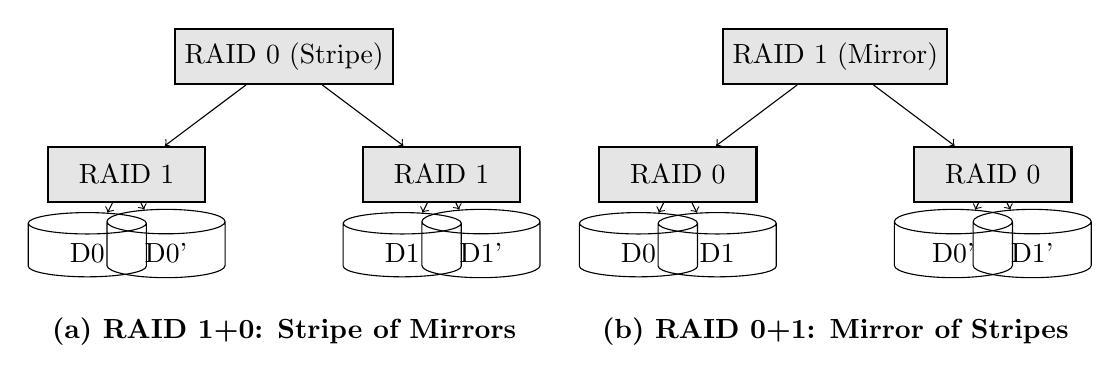
\begin{tikzpicture}[
    disk/.style={cylinder, shape border rotate=90, draw, minimum width=1.5cm, minimum height=0.5cm, aspect=0.4},
    ctrl/.style={rectangle, draw, thick, minimum width=2cm, minimum height=0.7cm, fill=gray!20}
]
    % RAID 1+0
    \node[ctrl] (c10_top) at (0, 2.5) {RAID 0 (Stripe)};
    \node[ctrl] (c10_m1) at (-2, 1) {RAID 1};
    \node[ctrl] (c10_m2) at (2, 1) {RAID 1};
    
    \node[disk] (d1) at (-2.5, 0) {D0};
    \node[disk] (d2) at (-1.5, 0) {D0'};
    \node[disk] (d3) at (1.5, 0) {D1};
    \node[disk] (d4) at (2.5, 0) {D1'};
    
    \draw[->] (c10_top) -- (c10_m1);
    \draw[->] (c10_top) -- (c10_m2);
    \draw[->] (c10_m1) -- (d1);
    \draw[->] (c10_m1) -- (d2);
    \draw[->] (c10_m2) -- (d3);
    \draw[->] (c10_m2) -- (d4);
    
    \node at (0, -1) {\textbf{(a) RAID 1+0: Stripe of Mirrors}};

    % RAID 0+1
    \node[ctrl] (c01_top) at (7, 2.5) {RAID 1 (Mirror)};
    \node[ctrl] (c01_s1) at (5, 1) {RAID 0};
    \node[ctrl] (c01_s2) at (9, 1) {RAID 0};
    
    \node[disk] (d5) at (4.5, 0) {D0};
    \node[disk] (d6) at (5.5, 0) {D1};
    \node[disk] (d7) at (8.5, 0) {D0'};
    \node[disk] (d8) at (9.5, 0) {D1'};
    
    \draw[->] (c01_top) -- (c01_s1);
    \draw[->] (c01_top) -- (c01_s2);
    \draw[->] (c01_s1) -- (d5);
    \draw[->] (c01_s1) -- (d6);
    \draw[->] (c01_s2) -- (d7);
    \draw[->] (c01_s2) -- (d8);
    
    \node at (7, -1) {\textbf{(b) RAID 0+1: Mirror of Stripes}};
\end{tikzpicture}
\caption{Architectural comparison of RAID 1+0 and RAID 0+1.}
\label{fig:nested_raid}
\end{figure}

\begin{table}[h!]
\centering
\caption{Comparison of Nested RAID Levels}
\label{tab:nested_raid}
\begin{tabular}{lll}
\toprule
\textbf{Attribute} & \textbf{RAID 1+0} & \textbf{RAID 0+1} \\
\midrule
\textbf{Usable Capacity} & $N/2 \times \text{DiskSize}$ & $N/2 \times \text{DiskSize}$ \\
\textbf{Performance} & Generally similar, high for all workloads. & Generally similar, high for all workloads. \\
\textbf{Reliability} & \textbf{Higher}. Survives multiple failures if they & \textbf{Lower}. A second failure on the \\
& occur in different mirrored pairs. & mirrored side causes total array failure. \\
\textbf{Rebuild Cost} & Lower. Only the failed disk's mirror is & Higher. The entire striped set must be \\
& needed for rebuild, reducing I/O load. & read to rebuild the mirror. \\
\bottomrule
\end{tabular}
\end{table}

\paragraph{Conclusion.} Due to its superior fault tolerance and more efficient rebuild process, \textbf{RAID 1+0 is almost always preferred over RAID 0+1} in modern system design.

\newpage
% -------------------------------------------------------------------------------------------------
\subsection{Parity-Based RAID: Levels 4, 5, and 6}
% -------------------------------------------------------------------------------------------------
These levels use parity for redundancy instead of mirroring, offering better storage efficiency.

\begin{itemize}
    \item \textbf{RAID 4:} Stripes data across $N-1$ disks and stores all parity information on a single, dedicated parity disk. This parity disk becomes a write bottleneck, as every write operation requires an update to it.
    \item \textbf{RAID 5:} Solves the RAID 4 bottleneck by distributing the parity blocks across all disks in the array, along with the data blocks. This balances the write load more effectively. It can tolerate a single disk failure.
    \item \textbf{RAID 6:} Extends RAID 5 by adding a second, independent parity block. This allows the array to tolerate the failure of any \textbf{two} disks, providing significantly higher reliability. This is critical for large arrays where the probability of a second failure occurring during the lengthy rebuild of a first failure is non-trivial.
\end{itemize}

The performance of these levels, particularly for writes, is more complex due to the "read-modify-write" penalty associated with updating parity information.

\newpage
% =================================================================================================
\section{Performance Analysis Formalism}
% =================================================================================================

To properly evaluate RAID performance, we must distinguish between sequential and random access patterns, as their impact on disk mechanics is vastly different.

% -------------------------------------------------------------------------------------------------
\subsection{Single Disk Baseline}
% -------------------------------------------------------------------------------------------------

Let's establish a baseline for a typical mechanical hard drive.
\begin{itemize}
    \item Average Seek Time ($T_{seek}$): 7 ms
    \item Rotational Delay ($T_{rotation}$): 3 ms (for a 10,000 RPM disk, avg. is half rotation)
    \item Transfer Rate ($R_{transfer}$): 50 MB/s
\end{itemize}

\subsubsection{Sequential Access Bandwidth (S)}
For a large sequential transfer (e.g., 10 MB), the mechanical overhead is paid only once.
\begin{equation}
    T_{total} = T_{seek} + T_{rotation} + T_{transfer} = 7ms + 3ms + \frac{10 \, \text{MB}}{50 \, \text{MB/s}} = 10ms + 200ms = 210ms
\end{equation}
The effective bandwidth, $S$, is:
\begin{equation}
    S = \frac{\text{Data Size}}{T_{total}} = \frac{10 \, \text{MB}}{0.21 \, \text{s}} \approx 47.6 \, \text{MB/s}
\end{equation}
\boxed{
    \text{For large transfers, } S \approx R_{transfer}
}

\subsubsection{Random Access Rate (R)}
For small random transfers (e.g., 10 KB), the mechanical overhead dominates each operation.
\begin{equation}
    T_{total} = T_{seek} + T_{rotation} + T_{transfer} = 7ms + 3ms + \frac{0.01 \, \text{MB}}{50 \, \text{MB/s}} = 10ms + 0.2ms = 10.2ms
\end{equation}
The effective bandwidth for a single request is low. A more useful metric is the number of I/O Operations Per Second (IOPS), which is $1/T_{total}$. The random access bandwidth, $R$, is:
\begin{equation}
    R = \frac{\text{Data Size}}{T_{total}} = \frac{10 \, \text{KB}}{0.0102 \, \text{s}} \approx 0.98 \, \text{MB/s}
\end{equation}
\boxed{
    \text{For small random transfers, } R \ll S
}

% -------------------------------------------------------------------------------------------------
\subsection{RAID Performance Summary}
% -------------------------------------------------------------------------------------------------
The following table summarizes the theoretical peak performance of various RAID levels in terms of the single-disk bandwidths $S$ and $R$.

\begin{table}[h!]
\centering
\caption{RAID Performance Characteristics ($N$ disks)}
\label{tab:perf_summary}
\begin{tabular}{lcccc}
\toprule
\textbf{RAID Level} & \textbf{Seq. Read} & \textbf{Seq. Write} & \textbf{Rand. Read} & \textbf{Rand. Write} \\
\midrule
RAID 0 & $N \times S$ & $N \times S$ & $N \times R$ & $N \times R$ \\
RAID 1 & $N \times S$ & $S$ & $N \times R$ & $R$ \\
RAID 1+0 & $N \times S$ & $\frac{N}{2} \times S$ & $N \times R$ & $\frac{N}{2} \times R$ \\
RAID 5 & $(N-1) \times S$ & $(N-1) \times S$ & $N \times R$ & $\frac{N}{4} \times R$ \textsuperscript{\textdagger} \\
\bottomrule
\end{tabular}
\caption*{\textsuperscript{\textdagger}\footnotesize{The random write performance for RAID 5 is significantly penalized by the read-modify-write cycle. A single logical write requires four physical I/O operations: read old data, read old parity, write new data, write new parity.}}
\end{table}

\end{document}
